%%%%
% -- Schedule and Budget breakdown and funding path
% --     FOBOS Keck White Paper 2019
%%%%

\section{Schedule, Budget, and Funding Path}
\label{sec:budget}

FOBOS development has borrowed heavily from the TMT Fiber-WFOS design
effort and has been supported by small grants listed in the table
below. WMKO 2018 white-paper funds have allowed for initial science
requirements and science team building. Remaining funds for
spectrograph design and sampling optimization will be used in the
coming year. A 2018 UCO mini-grant (K.~Bundy; {\it FIDDLES}, ongoing)
provides \$120k for design and prototyping of microlens-coupled fiber
systems in the context of FOBOS and other UCO instruments.

 % {\it FIDDLES} addresses a high-risk design component early on in FOBOS planning.



%  to demonstrate its throughput at
% Keck compared to lab measurements and to simultaneous observations
% with DEIMOS. The latter builds on UCO's ongoing investment in a
% fiber-testing facility needed for a number of internal projects has
% helped to further the FOBOS design.

% Early funding for FOBOS has been obtained as follows. Conceptual
% development of Fiber-WFOS for TMT provided the backbone of the
% current FOBOS design. Grants for targeted studies include: a 2016 UCO
% mini-grant (K.-G.~Lee) for initial collaboration development; 2017
% UCO mini-grants for microlens fore-optics conceptual development
% (K.-G.~Lee) and the sky-subtraction fidelity of existing fiber
% systems (K.~Bundy); 

A schematic budget and schedule, including existing funding sources,
is provided below. The Phase-A funding requested here, if made
available in Summer 2019, will prepare FOBOS for the Fall 2019 NSF
MSIP solicitation. This is an important opportunity to secure
Preliminary Design funding from an NSF-AST program and would put
FOBOS on track to compete for the NSF-wide MsRI-2 construction
funding in 2023. Should the MSIP proposal fail in 2020, we would try
again for (highly competitive) MsRI-1 design funding in 2021 and a
second MSIP one year later. This uncertainty motivates our request
for SSC approval to pursue multiple funding opportunities, including
those outside of the NSF such as private donors and foundations.

% In this scenario, it is unclear whether FOBOS could be ready for an MsRI-2 construction proposal in 2023 or would have to wait for 2025.  

A major goal of the Phase-A effort is to estimate the overall FOBOS
cost. At this stage, any estimate should be taken with a grain of
salt. The costing exercise for Fiber-WFOS was designed to compare
costs on equal footing of two early-phase WFOS concepts, {\it not} to
provide an accurate final budget number. The highest price-point
Fiber-WFOS considered (\$67M including contingency\footnote{TMT
requires certain assumptions for costing. Correcting a
later-discovered mistake on UCO labor rates while assuming that all
labor is performed at UCO increases these cost esimates by
$\approx$10\%.}) consisted of five spectrographs, an imager, and
management of international partners. A 4-spectrograph Fiber-WFOS was
evaluated at \$62M (see TMT.SEN.MGT.18.038.REL03). The FOBOS Team is
very much aware of WMKO's requirement to keep costs as low as
possible and to ensure that budgeting is as accurate as possible
before the Observatory can approve FOBOS's advancement to future
design stages.


% For comparison, a recent estimate of final DEIMOS costs in 2018 dollars came to \$22M.  Project costs from other facilities are hard to glean, but VLT-MUSE is widely thought to have cost \$100M and Subaru-PFS, \$80M.  

%  (2020)
% and MsRI-2 (2023) programs (see Table~1). 

% We intend to propose for
% FOBOS design funds via an MSIP solicitation expected in early 2020;
% if successful, this will fund the full instrument-design phase. The
% construction funding would then come from a MsRI-2 proposal in 2023.
% The duration of our Phase-A request, late 2019 to mid 2021, will
% allow for continued development between submitting our MSIP proposal
% and when the funding is made available. In the event that we are
% unsuccessful in the MSIP proposal, we will refocus Phase-A funding
% during the latter half of this proposal period toward preparation of
% an MsRI-1 proposal in 2021. Additional funding proposals for smaller
% grants (e.g., UCO mini-grant, NSF ATI) will be sought as necessary
% and available. These grants would target relatively self-contained
% design components of FOBOS's overall system. Other government funding
% and private funding is also being pursued as opportunities become
% available.

\begin{table}[h!]
\centering
\footnotesize
\caption{FOBOS Development Milestones}
\label{tab:milestones}
\vspace*{-10pt}
\begin{tabular}{l r r}
Milestone                     & Funding Level & Dates \\
\hline
\hline
CoD Mini Grant I              &  \$10k & FY2016 \\
CoD Mini Grant II             &  \$25k & FY2017 \\
CoD Mini Grant III            &  \$55k & FY2017 \\
LBNL workshop                 &        & 18 Jan 2018 \\
UCLA workshop                 &        & 4 May 2018 \\
WMKO Design                   &  \$40k & 8 Jun 2018 \\
WMKO Design Funding Window    &        & 1 Dec 2018 -- 30 Nov 2019 \\
CoD Mini Grant IV (FIDDLES)   & \$120k & FY2019 \\
FIDDLES Funding Window        &        & 10 Jan 2019 -- 11 Dec 2019 \\
\hline
MSRI-1 Design               & Declined & 19 Feb 2019 \\
WMKO Phase A                  & \request{} & 8 Jun 2019 \\
WMKO Phase A Funding Window   &        & 23 Sep 2019 -- 23 Jul 2021 \\
\hline
MSIP 2020 LOI, Pre-Proposal   &        & 1 Sep -- 18 Nov 2019 \\
MSIP 2020 Full Proposal       &   \$5M & 17 Apr 2020 \\
MSIP Funding Window           &        & 1 Sep 2020 -- 31 Aug 2024 \\
\hline
MSRI-1 Design pre-proposal (if no 2019 MSIP)    &  & Feb 2021 \\
MSIP 2021 pre-proposal (if no 2019 MSIP)        &  & Nov 2021 \\
\hline
MSRI-2 LOI, Pre-Proposal      &        & 16 Feb -- 13 Mar 2023 \\
MSRI-2 Full Proposal          & $>$\$30M & 4 Aug 2023 \\
MSRI-2 Funding window         &        & 1 Aug 2024 -- 31 Sep 2028 \\
\hline
\end{tabular}
\end{table}

\newpage

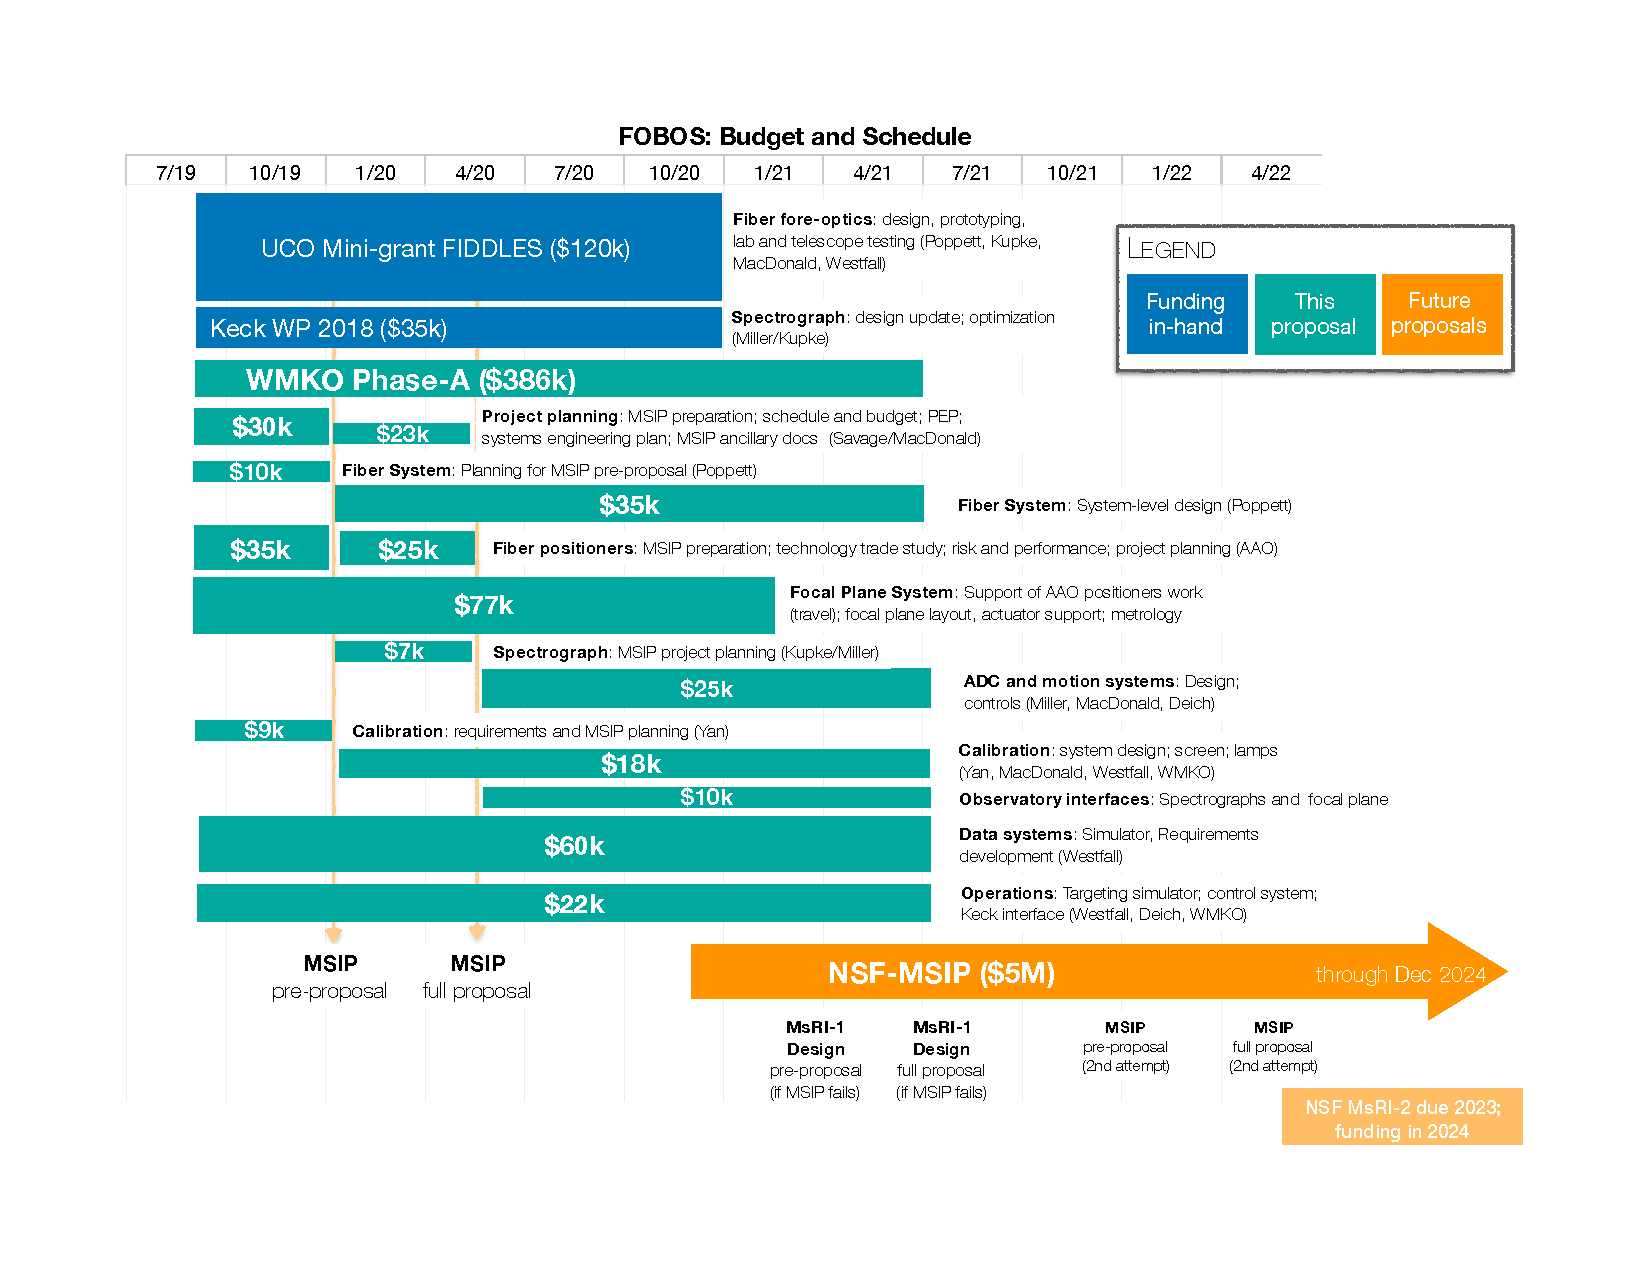
\includepdf[landscape=true]{figs/budget_schedule_schematic_v4.pdf}





